\documentclass[a4paper,10pt]{report}
\usepackage[utf8]{inputenc}
\usepackage{xcolor}   % for \textcolor
\usepackage{listings}
\usepackage{graphicx}

% Title Page
\title{Manuel d'utilisation et d'installation.}
\author{Yann Lederrey}


\begin{document}
\maketitle

\chapter{Manuel d'utilisation}
\section{Serveur}
Avant de démarrer le serveur veuillez vérifier que vous avez suivis l'installation de celui-ci (vous trouverez l'information dans la suite du document).\\
Pour démarrer le serveur exécutez la commande java -jar ds\_server.jar dans le terminal.\\
Cette application n'affiche des informations que dans le terminal, Ceci est 
normal et les informations affichées sont des informations de débug du au fait que nous ne sommes que en ALPHA.

\section{Client}
Avant de démarrer un client veuillez vérifier que vous avez suivis les étapes d'installation de celui-ci (vous trouverez l'information dans la suite du document).\\
Pour démarrer le serveur exécutez la commande java -jar ds\_client-1.0-SNAPSHOT-launcher.jars dans le terminal.\\
Sachez que afin d'avoir des questions à poser il faut jouer au mode histoire. Chaque question répondue juste vous sera ajoutée à votre liste personelle. Vous pourrez alors la 
poser dans le mode duel.\\
A la fin de chaque combat dans le mode histoire vous gagnez un item aléatoire. A la fin d'un combat en mode duel vous gagnez un item correspondant au type d'aversaire que vous avez battu.
\subsection{Acccueil}
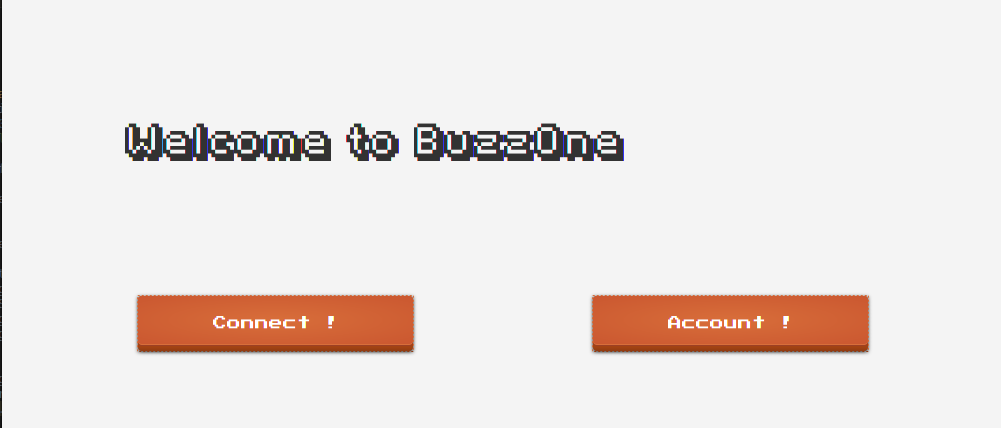
\includegraphics[scale=0.3]{images/AccountConnect.png}

\subsection{Création de compte}
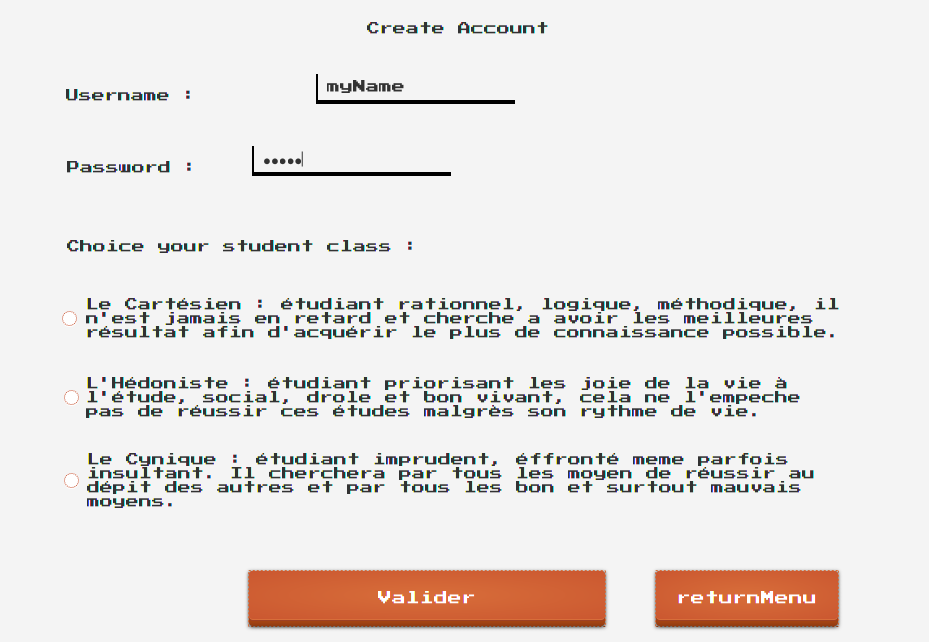
\includegraphics[scale=0.3]{images/account.png}
\begin{enumerate}
 \item Créer un compte : pour cela choisissez Account.
 \item Ajoutez un username et un mot de passe et choisissez votre classe. Les classes définissent seulement l'image de votre personnage ainsi que les 3 items de départ. (cf. rapport générale)
 \item Cliquez sur Valider.
\end{enumerate}

\subsection{Connexion}
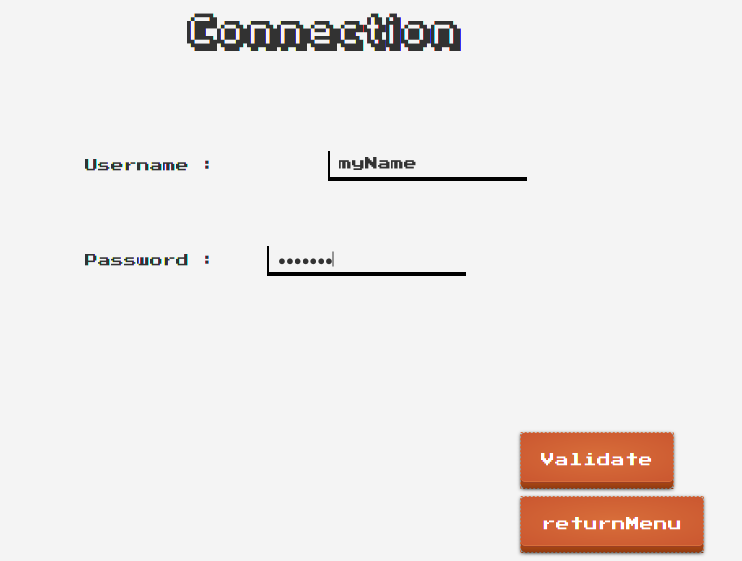
\includegraphics[scale=0.3]{images/connect.png}
\begin{enumerate}
 \item Se connecter : pour cela choisissez Connect.
 \item Donnez votre username et votre mot de passe.
 \item Cliquez sur Valider.
\end{enumerate}

\subsection{Menu de jeu}
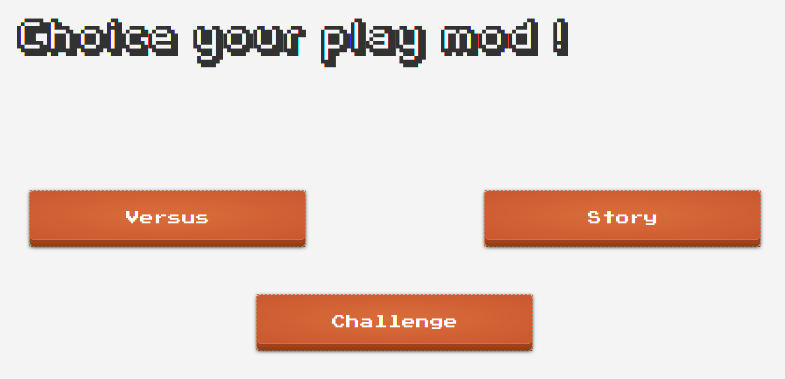
\includegraphics[scale=0.3]{images/hub.png}

\subsection{Mode joueur contre joueur}
\begin{enumerate}
 \item Vous voulez vous mettre en attente de défis : pour cela choisissez Versus. Il vous faut alors attendre que quelqu'un vous défie.
 \item Vous voulez défier quelqu'un en attente : pour cela choisissez Challenge.
\end{enumerate}

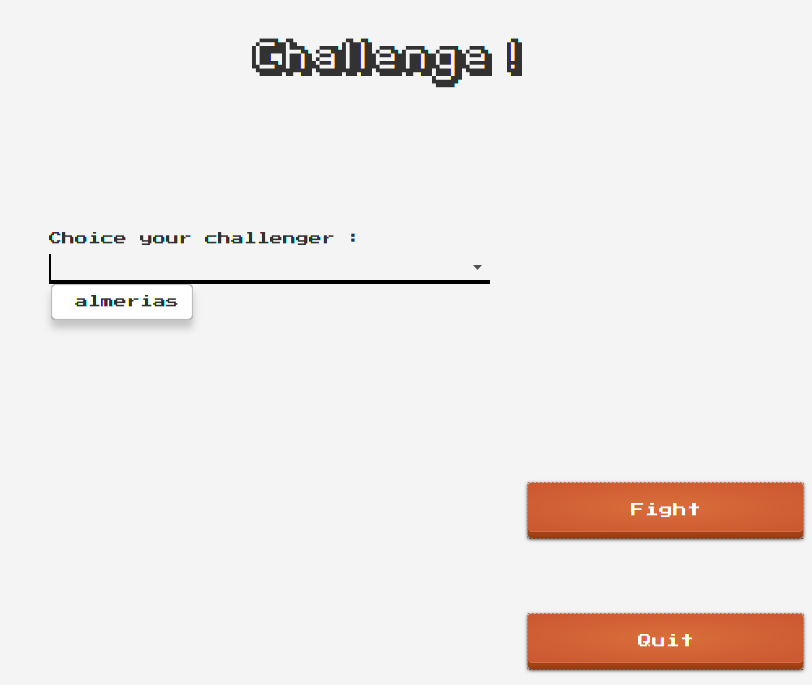
\includegraphics[scale=0.3]{images/challenge.png}

\begin{enumerate}
 \item choisissez votre adversaire dans la liste.
 \item Cliquez sur Fight
\end{enumerate}

\subsection{Mode histoire}
\begin{enumerate}
 \item Joueur en mode histoire : pour cela choisissez Story.
\end{enumerate}

\subsection{Combat}
Les combats fonctionnent en tour par tour. Le premier commence par poser ça question et l'autre répond. Vous avez la possiblité d'utiliser des items si vous en possédez.\\
Dans le cas du mode histoire vous ne pouvez pas poser de questions.\\
Lorsque vous répondez juste votre adversaire perd des points de vie, lorsque que votre adversaire répond faux il perd des points de vie.\\

\subsubsection{Poser une question}
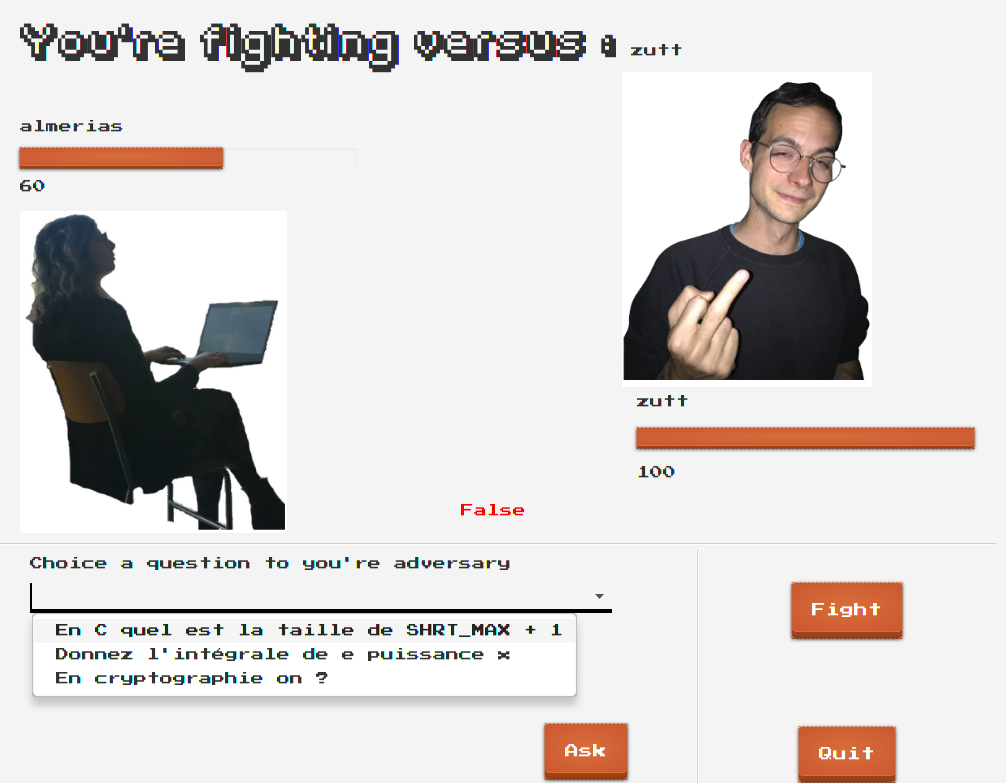
\includegraphics[scale=0.3]{images/poser.png}
\begin{enumerate}
 \item choisissez une question parmis celles à choix.
 \item Cliquez sur Ask.
 \item vous aurez de résultat de la dernière réponse donnée qui s'affichera (FALSE ou RIGHT).
 \item vous attendez alors que votre adversaire vous pose une question.
\end{enumerate}

\subsubsection{Répondre à une question}
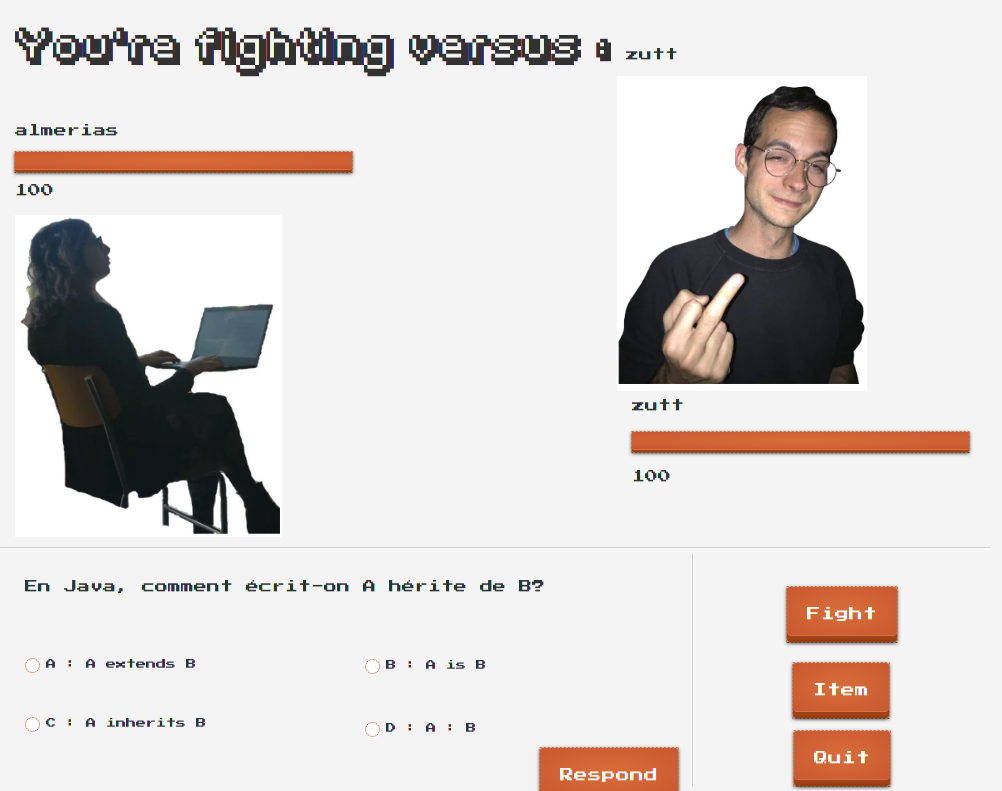
\includegraphics[scale=0.3]{images/repondre.png}
\begin{enumerate}
 \item Si vous sohaitez utiliser un item Cliquez sur le bouton Item.
 \item Sinon choisissez une réponses parmis celles à choix.
 \item Cliquez sur Answer.
 \item vous aurez de résultat de la dernière réponse donnée qui s'affichera (FALSE ou RIGHT).
 \item vous passerez en mode poser une question.
\end{enumerate}

\subsubsection{Utiliser un item}
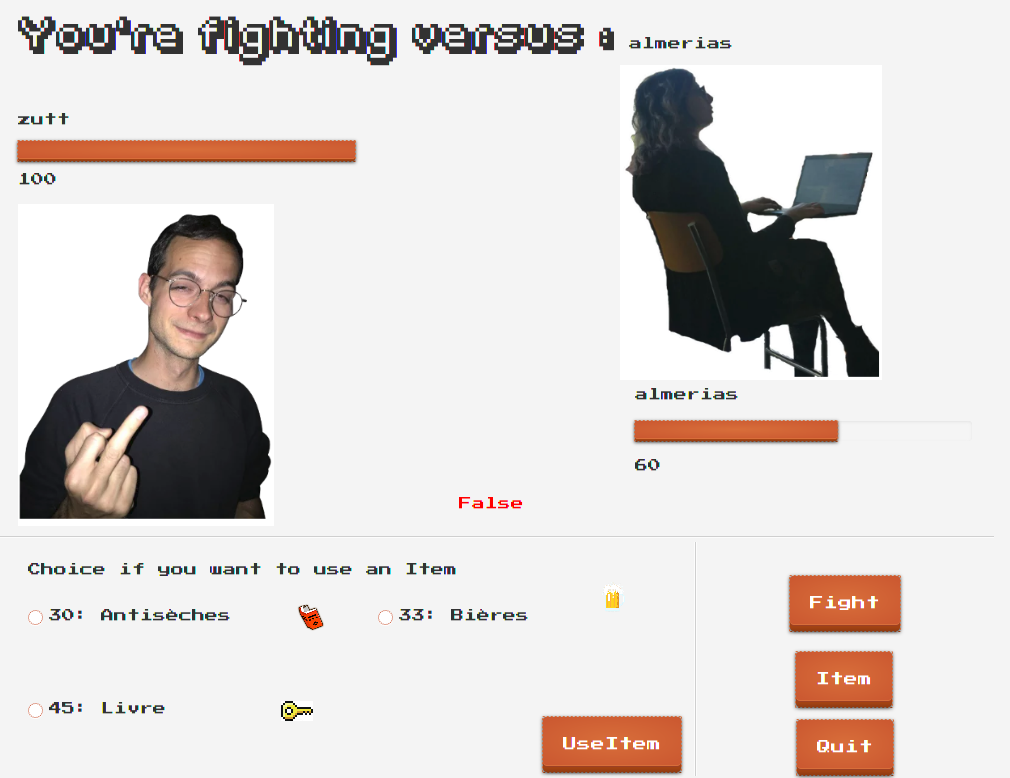
\includegraphics[scale=0.3]{images/item.png}
\begin{enumerate}
 \item Si vous sohaitez revenir au mode question cliquez sur Fight.
 \item Sinon choisissez un item parmis ceux disponible (nombre d'objet restant affiché).
 \item Cliquez sur UseItem.
 \item Revenez à la question avec le bouton Fight.
\end{enumerate}

\chapter{Manuel d'installation}

\section{Serveur}
\begin{enumerate}
 \item Vérifier que vous avez les fichiers de serveur comprenant :
\begin{itemize}
 \item Un fichier exécutable java : ds\_server.jar
 \item Un fichier questions.json
 \item Un dossier src contenant un dossier main contenant un fichier ds\_sb (base de données SQLLite
\end{itemize}
 \item Exécutez le fichier java avec la commande suivante : java -jar ds\_server.jar
\end{enumerate}
Cette application n'affiche des informations que dans le terminal, Ceci est 
 normal et les informations affichées sont des informations de débug du au fait que nous ne sommes que en ALPHA.
 
\subsection{Configuration}
La Configuration des questions du jeu et des professeurs se fait via l'édition du fichier questions.json.\\
Lorsque vous avez modifié le fichier questions il est obligatoire de redémarrer le serveur.\\
Pour ajouter une questions veuillez ajouter un ligne dans le tabeau Questions, la ligne doit impérativement respécter
la nomenclature suivante :

\begin{lstlisting}
{"id" : 1, "Question" : "En C quel est la taille de SHRT_MAX + 1", "RepOk" : "32,768", "rep2"  : "32,767", "rep3" : "−32,767", "rep4" : "0"}
\end{lstlisting}

\begin{itemize}
 \item id : numéro de la question (attention numéro unique).
 \item Question : Question que vous souhaitez poser.
 \item RepOk : réponse juste à votre question.
 \item Rep2 : une de vos réponses fausses.
 \item Rep3 : une de vos réponses fausses.
 \item Rep4 : une de vos réponses fausses.
 \item Si votre question n'est pas la dernière de la liste ajoutez une virgule à la fin.
\end{itemize}

Pour ajouter un professeur veuillez ajouter un ligne dans le tabeau Profs, la ligne doit impérativement respécter
la nomenclature suivante :

\begin{lstlisting}
{"id" : 1, "Prof" : "Miguel","pv" : 100, "niveau" : 1, "questions" : [13,14,15,22,23,24,42,43,44,45]}
\end{lstlisting}

\begin{itemize}
 \item id : numéro du professeur qui définira l'ordre dans lequel il arrive en mode histoire.
 \item Prof : Nom du professeur.
 \item pv : points de vie du professeur.
 \item niveau : niveau du professeur.
 \item questions : tableau d'id de question que le professeur peut demander.
 \item Si votre question n'est pas la dernière de la liste ajoutez une virgule à la fin.
\end{itemize}

\section{Client}
\begin{enumerate}
 \item Vérifier que vous avez les fichiers de client comprenant :
\begin{itemize}
 \item Un fichier exécutable java : ds\_client-1.0-SNAPSHOT-launcher.jar
 \item Un fichier de configuration config.properties
\end{itemize}
 \item Exécutez le fichier java avec la commande suivante : java -jar ds\_client-1.0-SNAPSHOT-launcher.jar
\end{enumerate}

\subsection{Configuration}
Afin que votre application client puisse contacter votre serveur vous devez lui préciser un adresse et un port.\\
Vous pouvez préciser cette information dans le fichier config.properties\\
De base de serveur écoute en localhost sur le port 4500.

\end{document}          
